\documentclass{bredelebeamer}
\usepackage{graphicx}
\usepackage{amsmath,amsfonts,amsthm}
\usepackage{hyperref}
\usepackage{setspace}
%\usepackage{media9} % for movies
%\usepackage{multimedia} % for movies
\usepackage{caption} % for figure caption
\usepackage{animate}
\usepackage[final]{listings} % for listing source code
\usefonttheme[onlymath]{serif} % make the equations look better
% define box for listing
\definecolor{myblue}{HTML}{4C72B0}
\definecolor{myred}{HTML}{C54E52}
\definecolor{mygreen}{HTML}{56A968}
\lstset{
      language=C++,
      basicstyle=\ttfamily,
      frame=single,
      columns=flexible,
      breaklines=true,
      commentstyle=\color{mygreen},
      keywordstyle = \color{myblue},
      stringstyle  = \color{orange},
      }
\usepackage[absolute,overlay]{textpos} 
\setlength{\parskip}{0.9em}
\setbeamertemplate{navigation symbols}{}
\newcommand*\dif{\mathop{}\!\mathrm{d}}
%%%%%%%%% some settings
\captionsetup[figure]{labelformat=empty} % remove the prefix 'figure' for figure caption
\captionsetup[table]{labelformat=empty} % remove the prefix 'table' for figure caption
\setbeamertemplate{headline}{} %%%%%%%%%%% remove header %%%%%%%%%%%
\setbeamerfont{frametitle}{size=\Large} %% title font size

%%%%%%%%%% title
\title[ ]{DAFoam Workshop 2022}
\subtitle{v3.0.0}

\author{Ping He and Bernardo Pacini \\ ~ \\June 8, 2022 }


\date[June 8, 2022]{}

\setbeamercolor{title}{fg=Black,bg=White!0}
\setbeamercolor{frametitle}{fg=Black,bg=White!0}
%gets rid of footer
%will override 'frame number' instruction above
%comment out to revert to previous/default definitions
\setbeamertemplate{footline}[page number]

\begin{document}

%---------------------------------------------------------------%
\begin{frame}
  \titlepage
\end{frame}

%---------------------------------------------------------------%


%---------------------------------------------------------------%
\begin{frame}{Objectives}

After this workshop, you should be able to
\begin{itemize}
  \setlength\itemsep{1em}
 \item Get familiar with the new features and interfaces in DAFoam v3
 \item Run aerodynamic \& aerostructural optimizations with DAFoam v3
 \item Modify/add DAFoam's C++ and Python codes for a new feature
\end{itemize}

\end{frame}
%---------------------------------------------------------------%

%---------------------------------------------------------------%
\begin{frame}{A few notes}

  \begin{itemize}
    \setlength\itemsep{1em}
   \item We assume you are familiar with DAFoam v2.
   \item This workshop has \textbf{hands-on} examples.
   \item \textbf{Stop} us at any time if you have questions.
   \item The online meeting will be \textbf{recorded}.
   \item All the materials are available at \url{https://github.com/dafoam/workshops}.
\end{itemize}
  
\end{frame}
%---------------------------------------------------------------%

%---------------------------------------------------------------%
\begin{frame}{Outline}
  \tableofcontents
\end{frame}
%---------------------------------------------------------------%

% ************************************************************************************
\section{DAFoam v3 Introduction}
\renewcommand{\arraystretch}{2}

%---------------------------------------------------------------%
\begin{frame}{}
  \center \Large DAFoam v3 Introduction
\end{frame}
%---------------------------------------------------------------%

%---------------------------------------------------------------%
\begin{frame}{What is DAFoam?}

  {\large DAFoam: \textbf{D}iscrete \textbf{A}djoint with Open\textbf{FOAM}}

  ~

  DAFoam develops an efficient discrete adjoint method to perform high-fidelity multidisciplinary design optimization. DAFoam has the following features:
  \center \normalsize
  \begin{itemize}
    \setlength\itemsep{1em}
    \item It uses a popular open-source package OpenFOAM (\url{www.openfoam.com}) for multiphysics analysis
    \item It implements a Jacobian-free discrete adjoint approach with competitive speed, scalability, and accuracy
    \item It has a convenient Python interface to couple with OpenMDAO (\url{www.openmdao.org}) for multidisciplinary design optimization
  \end{itemize}

\end{frame}
%---------------------------------------------------------------%

%---------------------------------------------------------------%
\begin{frame}{What is new in DAFoam v3?}
  DAFoam v3 is a major release that integrated DAFoam and OpenMDAO for multidisciplinary design optimization (MDO) through the OpenMDAO/Mphys interface

  \begin{itemize}
    \setlength\itemsep{1em}
    \item It developed a new Python interface (mphys/mphys\_dafoam.py) to Mphys and OpenMDAO for MDO
    \item Most of the settings are same as v2, but DAFoam v3 uses very different runScript.py because it is coupled with OpenMDAO.
    \item You need to update dependency versions for MDO in v3. Check the DAFoam website (\url{https://dafoam.github.io}).
    \item DAFoam v3 is compatible with all v2 run scripts.
  \end{itemize}
  
\end{frame}
%---------------------------------------------------------------%


% ************************************************************************************
\section{An OpenMDAO tutorial}
\renewcommand{\arraystretch}{2}

%---------------------------------------------------------------%
\begin{frame}{}
  \center \Large An OpenMDAO tutorial

  \normalsize
  For more advanced usage, refer to OpenMDAO's documentation at \\ 
  \url{https://openmdao.org/newdocs/versions/latest/main.html}
\end{frame}
%---------------------------------------------------------------%

%---------------------------------------------------------------%
\begin{frame}[fragile]{Optimizing a two-component system}
  \begin{figure}
    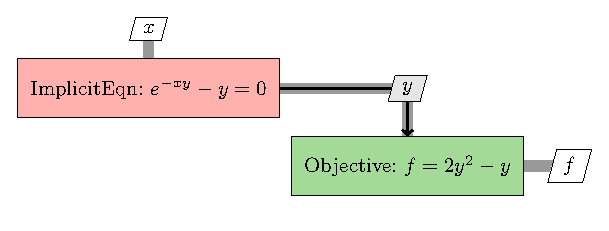
\includegraphics[width=\linewidth]{images/xdsm.pdf} 
    \caption{Design structure diagram for the two-component system. The red component is implicit and the green one is explicit. The design variable is $x$ and the objective function is $f$. $y$ is the solution from the implicit component and is passed to the explicit component as the input to compute $f$.}
  \end{figure}
\end{frame}
%---------------------------------------------------------------%


%---------------------------------------------------------------%
\begin{frame}[fragile]{Download DAFoam Docker image and examples}

  The most general way to run the above case is to use the DAFoam Docker image, which has OpenMDAO installed already.

  First, install Docker following this website: \\ \vspace{0.1in} \small \url{https://dafoam.github.io/mydoc_get_started_download_docker.html} \normalsize

  Once done, verify the installation by running:
  \footnotesize
  \lstset{ language=bash }
  \begin{lstlisting}
docker --version
  \end{lstlisting}
  \normalsize
     
  Then run this command to download the DAFoam Docker image: 

  \footnotesize
  \lstset{ language=bash }
  \begin{lstlisting}
docker pull dafoam/opt-packages:v3.0.0
  \end{lstlisting}
  \normalsize
  
  Finally, download the workshop examples at: \\ \vspace{0.1in}
  \small \texttt{\url{https://github.com/dafoam/workshops}}

\end{frame}
%---------------------------------------------------------------%


%---------------------------------------------------------------%
\begin{frame}[fragile]{Start a Docker container}

  If you use Linux or MacOS, open a terminal and use the \texttt{cd} command to go this folder on your local computer. If you put the workshops folder in the \$HOME directory, the command may look like:

  \footnotesize
  \begin{lstlisting}
cd $HOME/workshops/2022_Summer/examples/openmdao_example
  \end{lstlisting}
  \normalsize
  
  Then, run this command to start a Docker container:

  \footnotesize
  \begin{lstlisting}
docker run -it --rm -u dafoamuser --mount \
"type=bind,src=$(pwd),target=/home/dafoamuser/mount" \ 
-w /home/dafoamuser/mount dafoam/opt-packages:v3.0.0 bash
  \end{lstlisting}
  \normalsize

  If you use Windows, open the Prompt Command terminal, use the \texttt{cd} command to go to the above folder, and run this command: \\ \vspace{0.1in}

  \footnotesize
  \begin{lstlisting}
docker run -it --rm -u dafoamuser --mount \
"type=bind,src=%cd%,target=/home/dafoamuser/mount" \
-w /home/dafoamuser/mount dafoam/opt-packages:v3.0.0 bash
  \end{lstlisting}
  \normalsize

  Once in a Docker container, you should see something like:
  \footnotesize
  \lstset{ language=bash }
  \begin{lstlisting}
dafoamuser@cddb89839078:~/mount$ 
  \end{lstlisting}
  \normalsize

\end{frame}
%---------------------------------------------------------------%



%---------------------------------------------------------------%
\begin{frame}[fragile]{Run the case}

  Once in the docker container, use the \texttt{ls} command to check if you are in the correct directory. You should see something like this:

  \footnotesize
  \begin{lstlisting}
dafoamuser@cddb89839078:~/mount$ ls
n2.html  runScript.py  xdsm.pdf  xdsm.py
  \end{lstlisting}
  \normalsize

  Finally, you can run the case with this command:

  \footnotesize
  \begin{lstlisting}
python runScript.py
  \end{lstlisting}
  \normalsize

  Expected output:

  \footnotesize
  \begin{lstlisting}
dafoamuser@cddb89839078:~/mount$ python runScript.py 
Optimization terminated successfully    (Exit mode 0)
            Current function value: [0.87500003]
            Iterations: 11
            Function evaluations: 11
            Gradient evaluations: 11
Optimization Complete
-----------------------------------
f_opt: [0.87500003]
x_opt: [5.54015542]
  \end{lstlisting}
  \normalsize

\end{frame}
%---------------------------------------------------------------%


%---------------------------------------------------------------%
\begin{frame}[fragile]{An alternative option without Docker}

If you already have a Python 3 on your computer, you can directly run the OpenMDAO case without using the Docker. First, load your Python 3 environment, and run this command in your terminal to install OpenMDAO
  \footnotesize
  \lstset{ language=bash }
  \begin{lstlisting}
pip install openmdao==3.16.0
  \end{lstlisting}
  \normalsize
     
  Then go to the tutorial folder:

  \footnotesize
  \begin{lstlisting}
cd $HOME/workshops/2022_Summer/examples/openmdao_example
  \end{lstlisting}
  \normalsize

  And run the case:

  \footnotesize
  \lstset{ language=bash }
  \begin{lstlisting}
python runScript.py
  \end{lstlisting}
  \normalsize

\end{frame}
%---------------------------------------------------------------%

%---------------------------------------------------------------%
\begin{frame}[fragile]{N2 diagram}
  After the case is finished, you should see the N2 diagram (n2.html) for this case. The runScript.py file essential sets the components and their data transfer (connection) for the optimization.
  \begin{figure}
    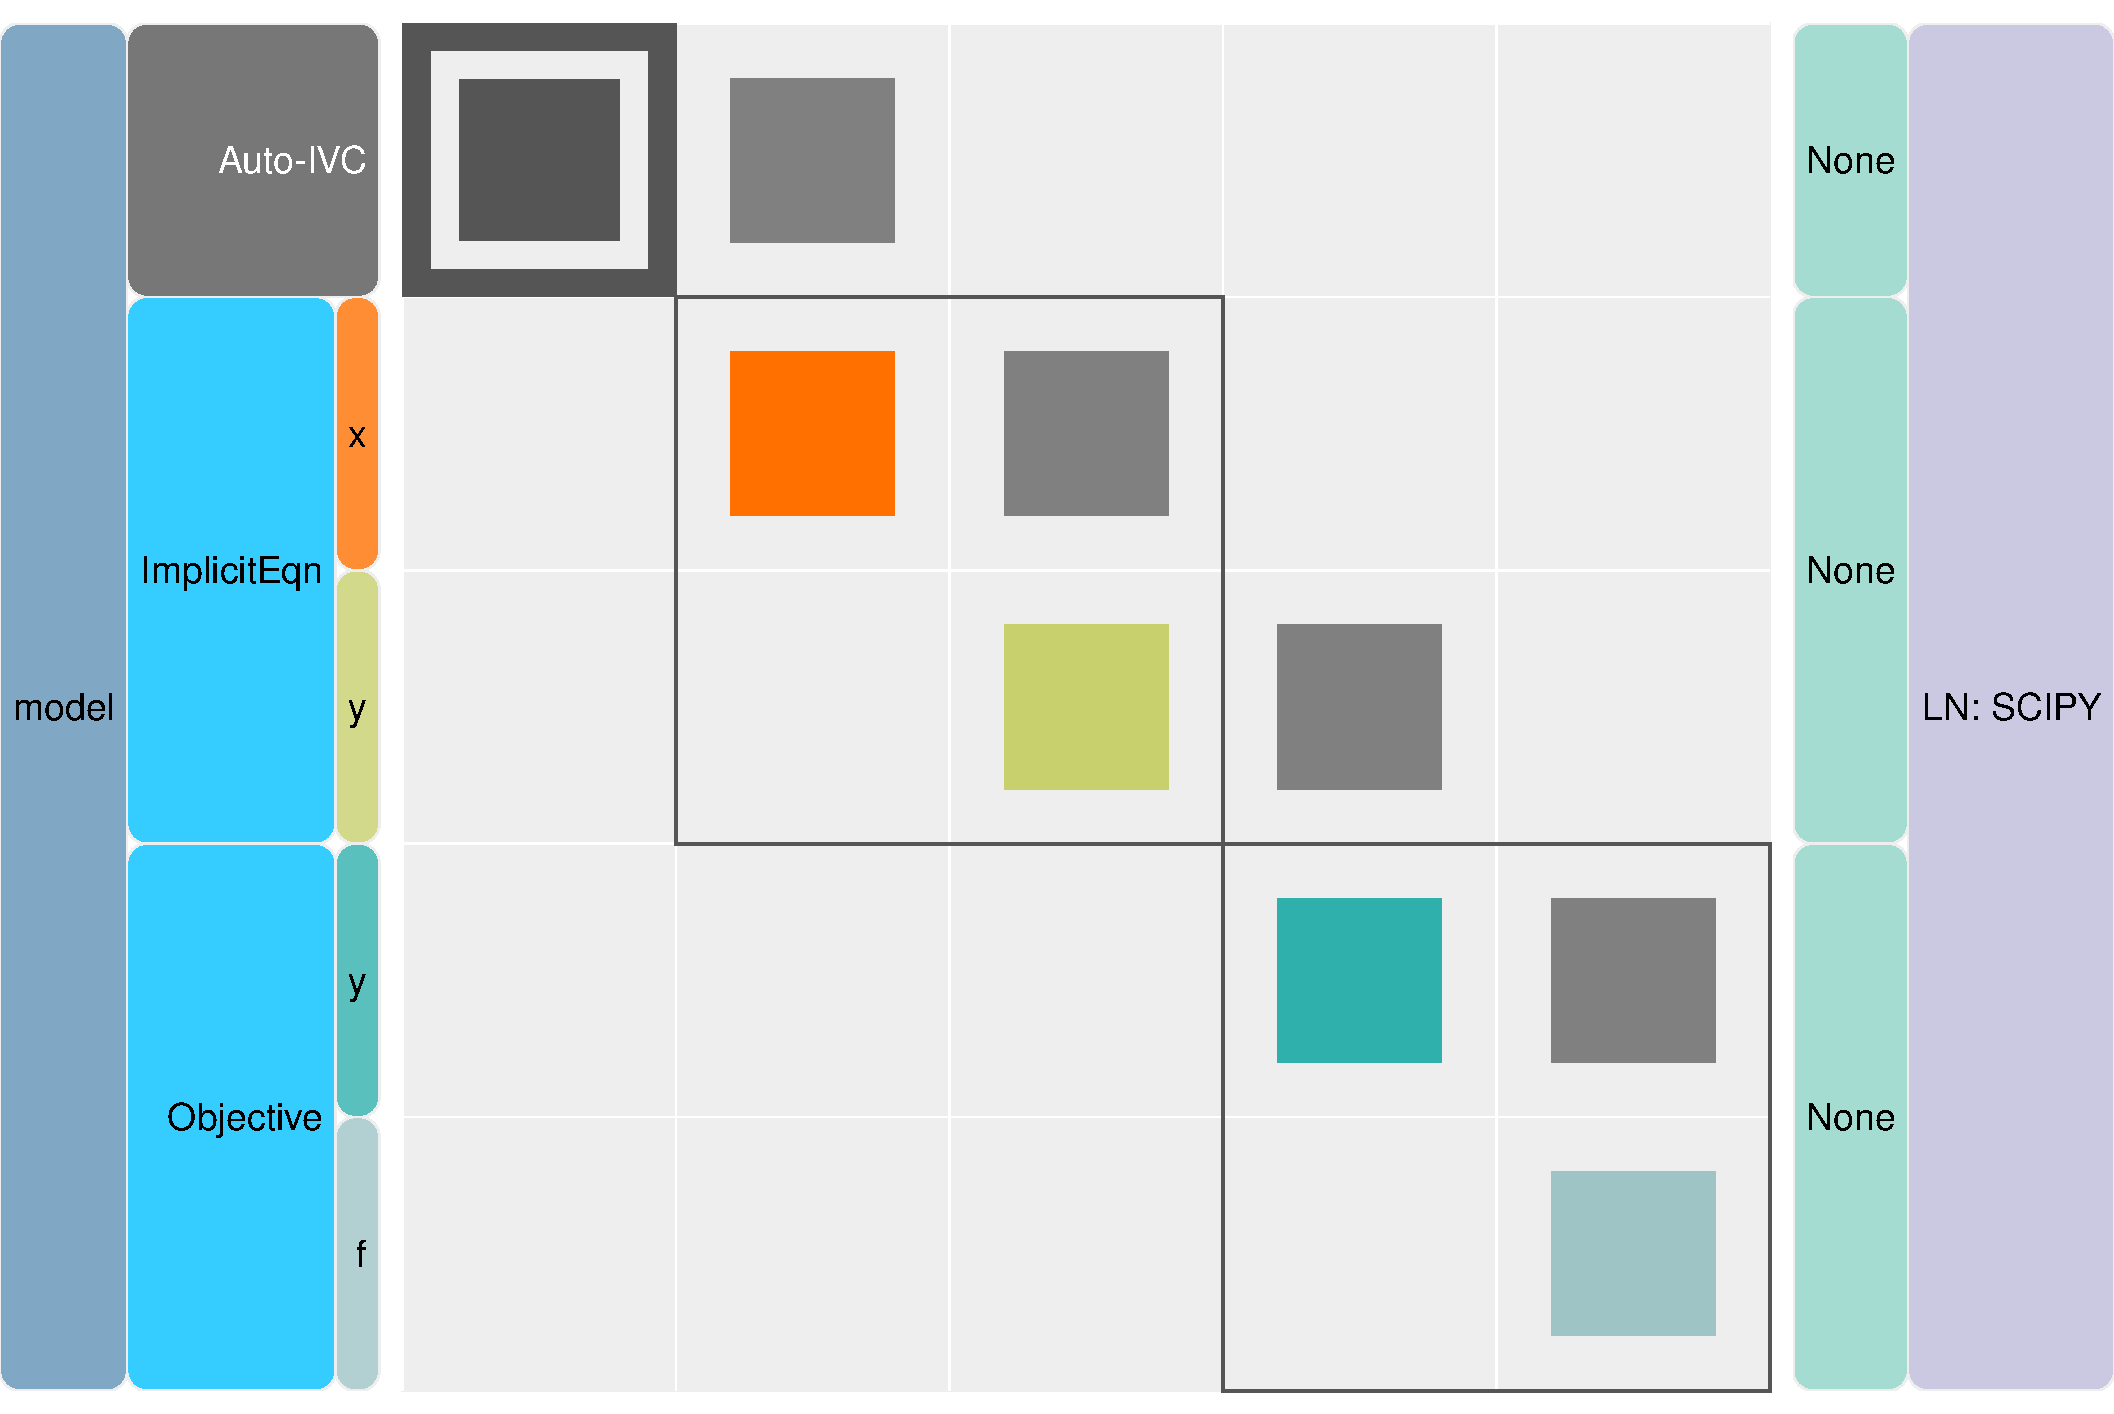
\includegraphics[width=0.8\linewidth]{images/example_n2.pdf} 
    \caption{The N2 diagram for the two-component optimization.}
  \end{figure}
\end{frame}
%---------------------------------------------------------------%


%---------------------------------------------------------------%
\begin{frame}[fragile]{runScript.py details (1/3)}
  \footnotesize
  \lstset{ language=python }
  \begin{lstlisting}
class ImplicitEqn(om.ImplicitComponent):
    def setup(self):
        # define input
        self.add_input("x", val=1.0)
        # define output
        self.add_output("y", val=1.0)

    def setup_partials(self):
        # Finite difference all partials.
        self.declare_partials("*", "*", method="fd")

    def apply_nonlinear(self, inputs, outputs, residuals):
        # get the input and output and compute the residual
        # R = e^(-x * y) - y
        # NOTE: we use [0] here because OpenMDAO assumes all inputs
        # and outputs are arrays. If the input is a scalar, OpenMDAO
        # will create an array that has size 1, so to get its value
        # we have to use [0]
        x = inputs["x"][0]
        y = outputs["y"][0]
        residuals["y"] = np.exp(-x * y) - y
  \end{lstlisting}
  \normalsize
\end{frame}
%---------------------------------------------------------------%

%---------------------------------------------------------------%
\begin{frame}[fragile]{runScript.py details (2/3)}
  \footnotesize
  \lstset{ language=python }
  \begin{lstlisting}
class ImplicitEqn(om.ImplicitComponent):
    def setup(self):
        # define input
        self.add_input("x", val=1.0)
        # define output
        self.add_output("y", val=1.0)

    def setup_partials(self):
        # Finite difference all partials.
        self.declare_partials("*", "*", method="fd")

    def apply_nonlinear(self, inputs, outputs, residuals):
        # get the input and output and compute the residual
        # R = e^(-x * y) - y
        # NOTE: we use [0] here because OpenMDAO assumes all inputs
        # and outputs are arrays. If the input is a scalar, OpenMDAO
        # will create an array that has size 1, so to get its value
        # we have to use [0]
        x = inputs["x"][0]
        y = outputs["y"][0]
        residuals["y"] = np.exp(-x * y) - y
  \end{lstlisting}
  \normalsize
\end{frame}
%---------------------------------------------------------------%


%---------------------------------------------------------------%
\begin{frame}[fragile]{runScript.py details (3/3)}
  \footnotesize
  \lstset{ language=python }
  \begin{lstlisting}
# create an OpenMDAO problem object
prob = om.Problem()
# now add the implicit component defined above to prob
prob.model.add_subsystem("ImplicitEqn", ImplicitEqn(), promotes=["*"])
# add the objective explicit component defined above to prob
prob.model.add_subsystem("Objective", Objective(), promotes=["*"],)
# set the linear/nonlinear equation solution for the implicit component
prob.model.nonlinear_solver = om.NewtonSolver(solve_subsystems=False)
prob.model.linear_solver = om.ScipyKrylov()
# set the design variable and objective function
prob.model.add_design_var("x", lower=-10, upper=10)
prob.model.add_objective("f", scaler=1)
# setup the optimizer
prob.driver = om.ScipyOptimizeDriver()
prob.driver.options["optimizer"] = "SLSQP"
# setup the problem
prob.setup()
# write the n2 diagram
om.n2(prob, show_browser=False, outfile="n2.html")
# run the optimization
prob.run_driver()
  \end{lstlisting}
  \normalsize
\end{frame}
%---------------------------------------------------------------%

%---------------------------------------------------------------%
\begin{frame}[fragile]{Summary}
  \begin{itemize}
    \setlength\itemsep{1em}
   \item To use OpenMDAO for optimizations, one needs to write classes for each component in the system, define their inputs and outputs, and implement the way to compute the outputs (explicit components) or residuals (implicit components). 
   \item Then one needs to add these components to the optimization problem in the run script, set their connection, set the design variables, objective and constraint functions, and run the optimization.
   \item A new open-source interface Mphys was recently developed (\url{https://github.com/openmdao/mphys}) to rewrite the MACH-Aero modules' interfaces (e.g., pyGeo, IDWarp) into the OpenMDAO component format. 
   \item DAFoam v3 has a Python interface to OpenMDAO/Mphys (dafoam/mphys/mphys\_dafoam.py). So to run optimizations with DAFoam v3, one needs to use the new run script that sets the components, data transfer, design variables, objective and constraint functions in the optimization.
  \end{itemize}
\end{frame}
%---------------------------------------------------------------%


% ************************************************************************************
\section{Aerodynamic optimization}
\renewcommand{\arraystretch}{2}

%---------------------------------------------------------------%
\begin{frame}{}
  \center \Large Aerodynamic optimization
\end{frame}
%---------------------------------------------------------------%



%---------------------------------------------------------------%
\begin{frame}{Summary of the NACA0012 subsonic case}

  \begin{table}
    \renewcommand{\arraystretch}{1.5}
    \small
    \centering
    \label{tab:implemented_models}
    \begin{tabular}{llllllllllll}
    \hline
    Optimizer   & IPOPT \\
    Flow and adjoint solvers  & DARhoSimpleFoam  \\
    Geometry  & NACA0012 \\
    Mesh  & 4\,032 cells\\
    Objective function  & $C_d$ \\
    Design variables & 20 FFDs and $\alpha$ \\
    Constraint & $C_l=0.5$, thickness, volume, TE/LE \\
    $U_\infty$  & 100 m/s \\
    $Re$  & 6.7$\times10^6$\\
    Turbulence Model  & Spalart--Allmaras\\
     \hline
    \end{tabular}
  \end{table}

  You can find the case settings in workshops/2022\_Summer/examples/naca0012.
\end{frame}
%---------------------------------------------------------------%


%---------------------------------------------------------------%
\begin{frame}[fragile]{Run the case}

  First, use the \texttt{cd} command to go the workshop folder on your local computer. The command may look like:

  \footnotesize
  \begin{lstlisting}
cd $HOME/workshops/2022_Summer/examples/naca10012
  \end{lstlisting}
  \normalsize
  
  Use the command in Slide 11 to start a Docker container. Then, use the \texttt{ls} command to check if you are in the correct directory.
  \footnotesize
  \lstset{ language=bash }
  \begin{lstlisting}
dafoamuser@bd114f3f7c94:~/mount$ ls
0.orig       FFD       genAirFoilMesh.py  preProcessing.sh  runScript.py
Allclean.sh  constant  paraview.foam      profiles          system
  \end{lstlisting}
  \normalsize

  Next, run this command to generate the mesh:
  \footnotesize
  \lstset{ language=bash }
  \begin{lstlisting}
./preProcessing.sh
  \end{lstlisting}
  \normalsize

  Finally, run the optimization with 2 cores.
  \footnotesize
  \lstset{ language=bash }
  \begin{lstlisting}
mpirun -np 2 python runScript.py
  \end{lstlisting}
  \normalsize

\end{frame}
%---------------------------------------------------------------%



% ************************************************************************************
\section{Aerostructural optimization}
\renewcommand{\arraystretch}{2}

%---------------------------------------------------------------%
\begin{frame}{}
  \center \Large Aerostructural optimization
\end{frame}
%---------------------------------------------------------------%


% ************************************************************************************
\section{Add new features to DAFoam}
\renewcommand{\arraystretch}{2}

%---------------------------------------------------------------%
\begin{frame}{}
  \center \Large DAFoam code structure
\end{frame}
%---------------------------------------------------------------%

%---------------------------------------------------------------%
\begin{frame}[plain]{}
  \Huge \centering
  Thank you!
\end{frame}
%---------------------------------------------------------------%

\end{document}
